\documentclass[12pt]{standalone}
\usepackage{amsmath, relsize, tikz}
\usepackage{xcolor}
\usepackage{pgffor} % LATEX
\input pgffor.tex % plain TEX
\usetikzlibrary{matrix}
\usetikzlibrary{knots}
\usetikzlibrary{intersections,backgrounds}
\begin{document}
    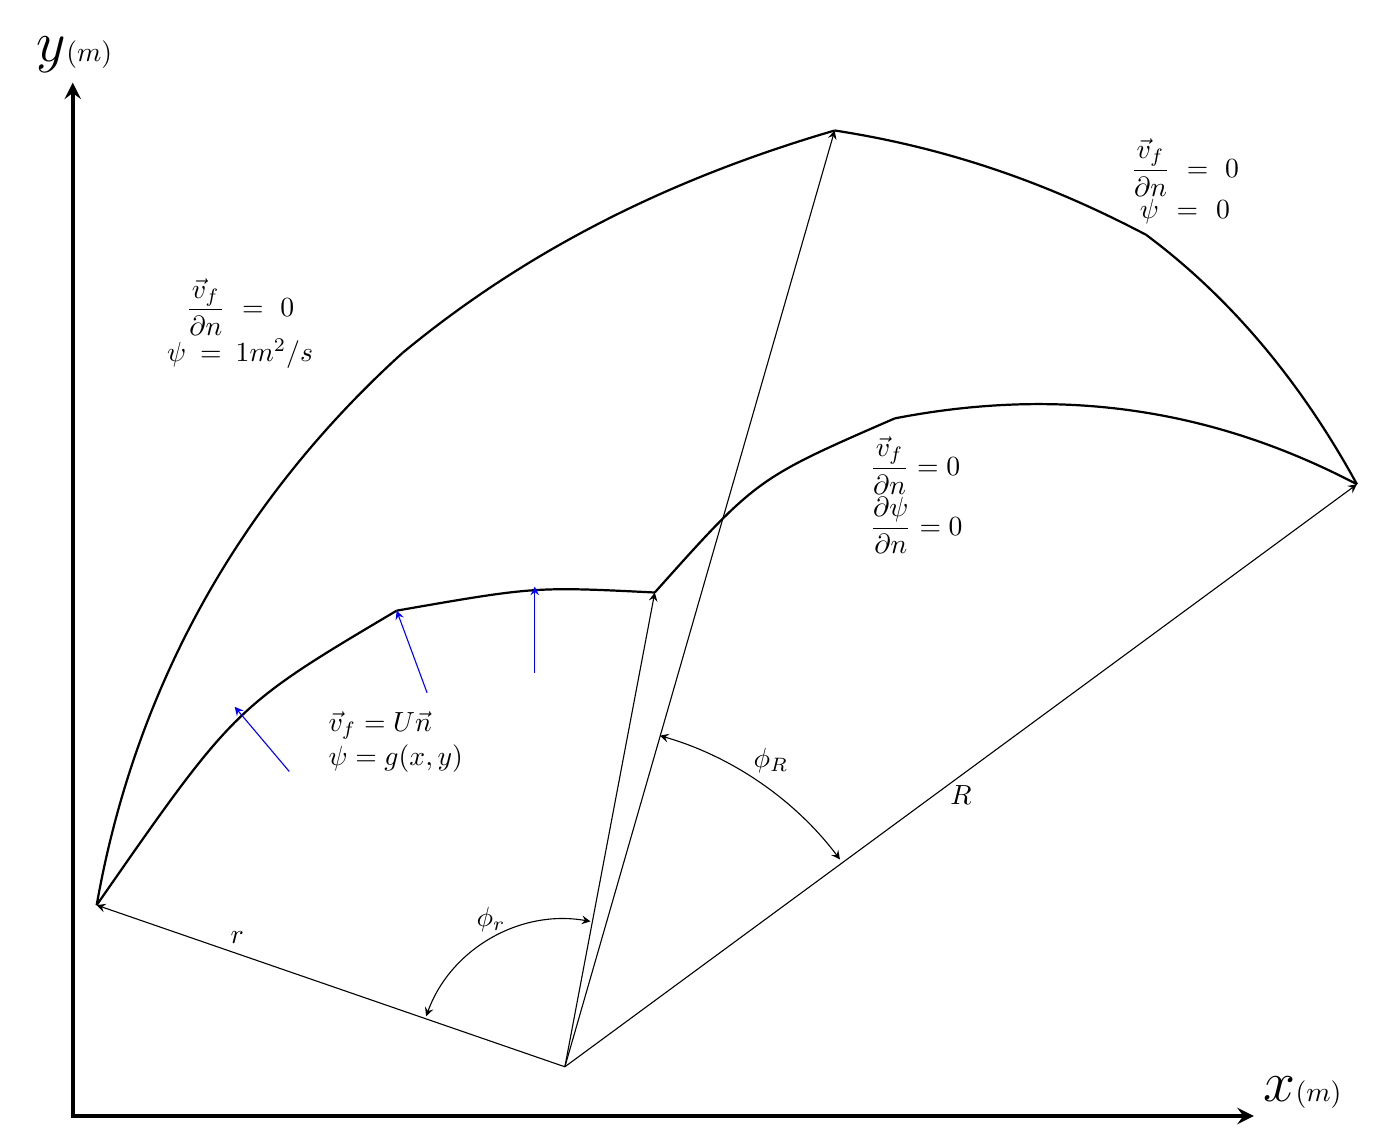
\begin{tikzpicture}[scale=12.5, >=stealth]
        \draw [<->, ultra thick] (0.0,1.0) -- (0.0,-0.05) -- (1.2,-0.05);
        \node [above left] at (0.05,1.0) {{\huge $y$}{$(m)$}};
        \node [below right] at (1.2,0.0) {{\huge $x$}{$(m)$}};

        \node [above left, text width=3cm, align=center] at (0.3, 0.7) {$\dfrac{\vec{v}_f}{\partial n} = 0$\\$\psi = 1m^2/s$};
        \node [right, text width=3cm, align=center] at (1.0, 0.9) {$\dfrac{\vec{v}_f}{\partial n} = 0$\\$\psi = 0$};
        \node [right, text width=3cm] at (0.25, 0.33) {$\vec{v}_f = U \vec{n}$\\$\psi = g(x,y)$};
        \node [below right, text width=3cm] at (0.8, 0.65) {$\dfrac{\vec{v}_f}{\partial n} = 0$\\$\dfrac{\partial \psi}{\partial n} = 0$};

        \draw [thick] (0.5+-0.475696, 0.16425) .. controls (0.5+-0.335515, 0.365799) .. (0.5+-0.170879, 0.463447);
        \draw [thick] (0.5+-0.170879, 0.463447).. controls (0.5+-0.0306224, 0.487911) .. (0.5+0.0913384, 0.481878);

        \draw [thick] (0.5+0.0913384, 0.481878) .. controls (0.5+0.194936, 0.597761) .. (0.5+0.335177, 0.658783);
        \draw [thick] (0.5+0.335177, 0.658783) .. controls (0.5+0.524198, 0.695431) and (0.5+0.676666, 0.658877) ..
        (0.5+0.80475, 0.591832);

        \draw [thick] (0.5+0.80475, 0.591832) .. controls (0.5+0.746361, 0.698382) and (0.5+0.674591, 0.782751) ..
        (0.5+0.590407, 0.845373);
        \draw [thick] (0.5+0.590407, 0.845373) .. controls (0.5+0.512491, 0.886172) and (0.5+0.409811, 0.930426) ..
        (0.5+0.274126, 0.951272);

        \draw [thick] (0.5+0.274126, 0.951272) .. controls (0.5+0.127821, 0.908513) and (0.5+-0.0245825, 0.84136) ..
        (0.5+-0.164765, 0.725434);
        \draw [thick] (0.5+-0.164765, 0.725434) .. controls (0.5+-0.292753, 0.609514) and (0.5+-0.428851, 0.429716) ..
        (0.5+-0.475696, 0.16425);

        \draw [->, blue] (0.5+-0.0306224, 0.4) -- (0.5+-0.0306224, 0.487911);
        \draw [->, blue] (0.36, 0.38) -- (0.5+-0.170879, 0.463447);
        \draw [->, blue] (0.22, 0.3) -- (0.5+-0.335515, 0.365799);

        \draw [->] (0.5, 0.0) -- (0.5+-0.475696, 0.16425) node [pos=0.7, above] {$r$};
        \draw [->] (0.5, 0.0) -- (0.5+0.0913384, 0.481878);
        \draw [<->] (0.5, 0.0)++(80:0.15) arc (80:160:0.15) node [midway, yshift=7.0] {$\phi_r$};

        \draw [->] (0.5, 0.0) -- (0.5+0.80475, 0.591832) node [midway, below] {$R$};
        \draw [->] (0.5, 0.0) -- (0.5+0.274126, 0.951272);
        \draw [<->] (0.5, 0.0)++(37:0.35) arc (37:74:0.35) node [midway, xshift=4.0, yshift=8.0] {$\phi_R$};
    \end{tikzpicture}
\end{document}

